% ============================================================
%  SECCIÓN 6 — Caso Real: Plataforma Tu Boleta + Santa Fe
%  Aplicación del modelo M/M/k/k (Erlang B) a la venta de
%  entradas online para partidos de fútbol. Listo para \input{}.
% ============================================================

\section{Actividad 6: Caso Real --- Plataforma \emph{Tu Boleta} y Rechazos de Compra}

\subsection*{Descripción del escenario}

Consideremos la plataforma web colombiana \textbf{Tu Boleta}, un servicio de venta de
entradas para conciertos, cine, teatro y eventos deportivos ---incluyendo partidos de
fútbol de equipos como el \textbf{Independiente Santa Fe}.

Cuando un hincha quiere comprar una entrada para un partido, su petición HTTP llega a un
balanceador de carga (\textit{Load Balancer}) que la distribuye entre varias instancias
del servicio (\textit{back-end}) encargadas de procesar la compra. Este modelo de arquitectura es estándar en clústeres de centros de datos y sistemas de orquestación modernos~\cite{greenberg2008, burns2016}.

En este sistema, cada instancia (servidor) puede atender \textbf{exactamente una} petición
de compra a la vez. Si un hincha llega mientras todas las instancias están ocupadas
procesando otras compras, el balanceador no lo deja esperar en una cola: le responde de
inmediato con un mensaje de error indicando que no hay capacidad disponible (equivalente
a un HTTP~503 \texttt{Service Unavailable}). Esto modela de forma directa el sistema
M/M/k/k.

\begin{figure}[H]
\centering
\begin{tikzpicture}[
    node distance=1.8cm,
    box/.style={
        rectangle, draw, rounded corners, thick,
        minimum width=3cm, minimum height=0.9cm,
        fill=blue!8, font=\small, align=center
    },
    inst/.style={
        rectangle, draw, thick, rounded corners,
        minimum width=2.6cm, minimum height=0.75cm,
        fill=green!12, font=\small
    },
    bloq/.style={
        rectangle, draw, dashed, thick, rounded corners,
        minimum width=2.6cm, minimum height=0.75cm,
        fill=red!10, font=\small
    },
    arr/.style={-{Stealth}, thick}
]
    \node[box] (usu) {Hinchas\\(Peticiones HTTP)};
    \node[box, right=2.2cm of usu] (lb) {Load\\Balancer};
    \node[inst, above right=0.5cm and 2.2cm of lb] (i1) {Instancia 1 (ocupada)};
    \node[inst, right=2.2cm of lb] (i2) {Instancia 2 (ocupada)};
    \node[inst, below right=0.5cm and 2.2cm of lb] (i3) {\(\vdots\) Instancia k (ocupada)};
    \node[bloq, below=1.8cm of lb] (blk) {\shortstack{Error 503:\\No hay cupo}};

    \draw[arr] (usu) -- (lb) node[midway, above] {$\lambda$};
    \draw[arr] (lb) -- (i1);
    \draw[arr] (lb) -- (i2);
    \draw[arr] (lb) -- (i3);
    \draw[arr, red!70, dashed] (lb) -- (blk)
        node[midway, right] {\footnotesize sistema lleno};
    \node[above=0.1cm of i1, font=\footnotesize, text=gray] {$\mu$ (exp.)};
\end{tikzpicture}
\caption{%
    Arquitectura de la plataforma \emph{Tu Boleta} modelada como sistema M/M/k/k.
    El Load Balancer distribuye peticiones de compra; las instancias son los $k$ servidores.
    Cuando todas están ocupadas, la respuesta es un rechazo inmediato (503).
}
\label{fig:tu_boleta}
\end{figure}

\subsection*{Correspondencia con el modelo M/M/k/k}

La analogía entre la plataforma \emph{Tu Boleta} (vendiendo entradas para Santa Fe) y
el modelo M/M/k/k se establece formalmente en la Tabla~\ref{tab:analogia_tuboleta}.

\begin{table}[H]
\centering
\caption{Correspondencia entre \emph{Tu Boleta} (venta de entradas Santa Fe) y el modelo M/M/k/k.}
\label{tab:analogia_tuboleta}
\begin{tabular}{ll}
\toprule
\textbf{Elemento del modelo M/M/k/k} & \textbf{Elemento en \emph{Tu Boleta}} \\
\midrule
Tasa de llegadas $\lambda$ & Hinchas intentando comprar entrada (req/min) \\
Tiempo de servicio $\sim \mathrm{Exp}(\mu)$ & Tiempo de procesamiento de cada compra \\
$k$ servidores en paralelo & $k$ instancias del back-end activas \\
Capacidad $=k$ (sin cola) & Sin fila de espera; rechazo inmediato \\
Estado $n$: ocupación del sistema & Instancias atendiendo compras \\
Bloqueo (prob.\ $B(k,a)$) & Hinchas que se quedan sin entrada \\
Carga ofrecida $a=\lambda/\mu$ & Intensidad de tráfico en Erlangs \\
\bottomrule
\end{tabular}
\end{table}

\subsection*{Escenarios de partido}

Se analizan cuatro escenarios representativos del calendario del
\textbf{Independiente Santa Fe}, ordenados por intensidad de demanda:

\begin{enumerate}
    \item \textbf{Partido de Liga regular:} partido contra rival de media tabla,
          con afluencia moderada de hinchas.
    \item \textbf{Clásico vs Millonarios:} el partido más importante del año,
          con demanda extremadamente alta.
    \item \textbf{Final de Copa:} partido de eliminación directa, con afluencia
          masiva de hinchas.
    \item \textbf{Súper-clásico (Clausura):} definición del torneo contra el
          máximo rival, con demanda histórica.
\end{enumerate}

Los parámetros de cada escenario se definen como sigue:

\begin{table}[H]
\centering
\caption{Parámetros de los escenarios de venta de entradas Santa Fe en \emph{Tu Boleta}.}
\label{tab:escenarios_tuboleta}
\begin{tabular}{lccccc}
\toprule
\textbf{Escenario} & $k$ & $\lambda$ (req/min) & $\mu$ (req/min) & $a$ (Erlangs) & $B(k,a)$ \\
\midrule
Partido de Liga regular & 5 & 20 & 4.0 & 5.00 & 0.2849 \\
Clásico vs Millonarios & 10 & 60 & 3.0 & 20.00 & 0.5380 \\
Final de Copa & 15 & 100 & 2.0 & 50.00 & 0.7080 \\
Súper-clásico (Clausura) & 20 & 150 & 2.5 & 60.00 & 0.6744 \\
\bottomrule
\end{tabular}
\end{table}

\subsection*{Validación de los supuestos del modelo}

\paragraph{Supuesto de llegadas Poisson.}
En una plataforma web como \emph{Tu Boleta} con miles de hinchas independientes intentando
comprar al mismo tiempo, el teorema de superposición de Poisson garantiza que la suma de
muchos procesos de llegadas de baja intensidad converge a un proceso Poisson. Dado que
ningún hincha individual domina el tráfico, el supuesto se sostiene desde el punto de
vista teórico.

\paragraph{Supuesto de tiempos de servicio exponenciales.}
El tiempo de procesamiento de una compra depende de factores heterogéneos (verificación de
pago, consulta a inventario de sillas, envío de correo de confirmación, generación de QR),
lo que justifica la aproximación exponencial. Además, la fórmula de Erlang~B es
\emph{insensible} a la distribución del tiempo de servicio~\cite{bonald2003}: solo necesita que la media
sea $1/\mu$.

\subsection*{Análisis de las trazas simuladas}

Para validar empíricamente el modelo se generaron datos sintéticos siguiendo la misma
metodología de las Actividades~4 y~5 del curso: generar interarribos y tiempos de servicio
exponenciales, y luego graficar su PDF, CDF y QQ-plot frente a la distribución teórica.

\begin{figure}[H]
\centering
\begin{subfigure}{0.48\textwidth}
    \centering
    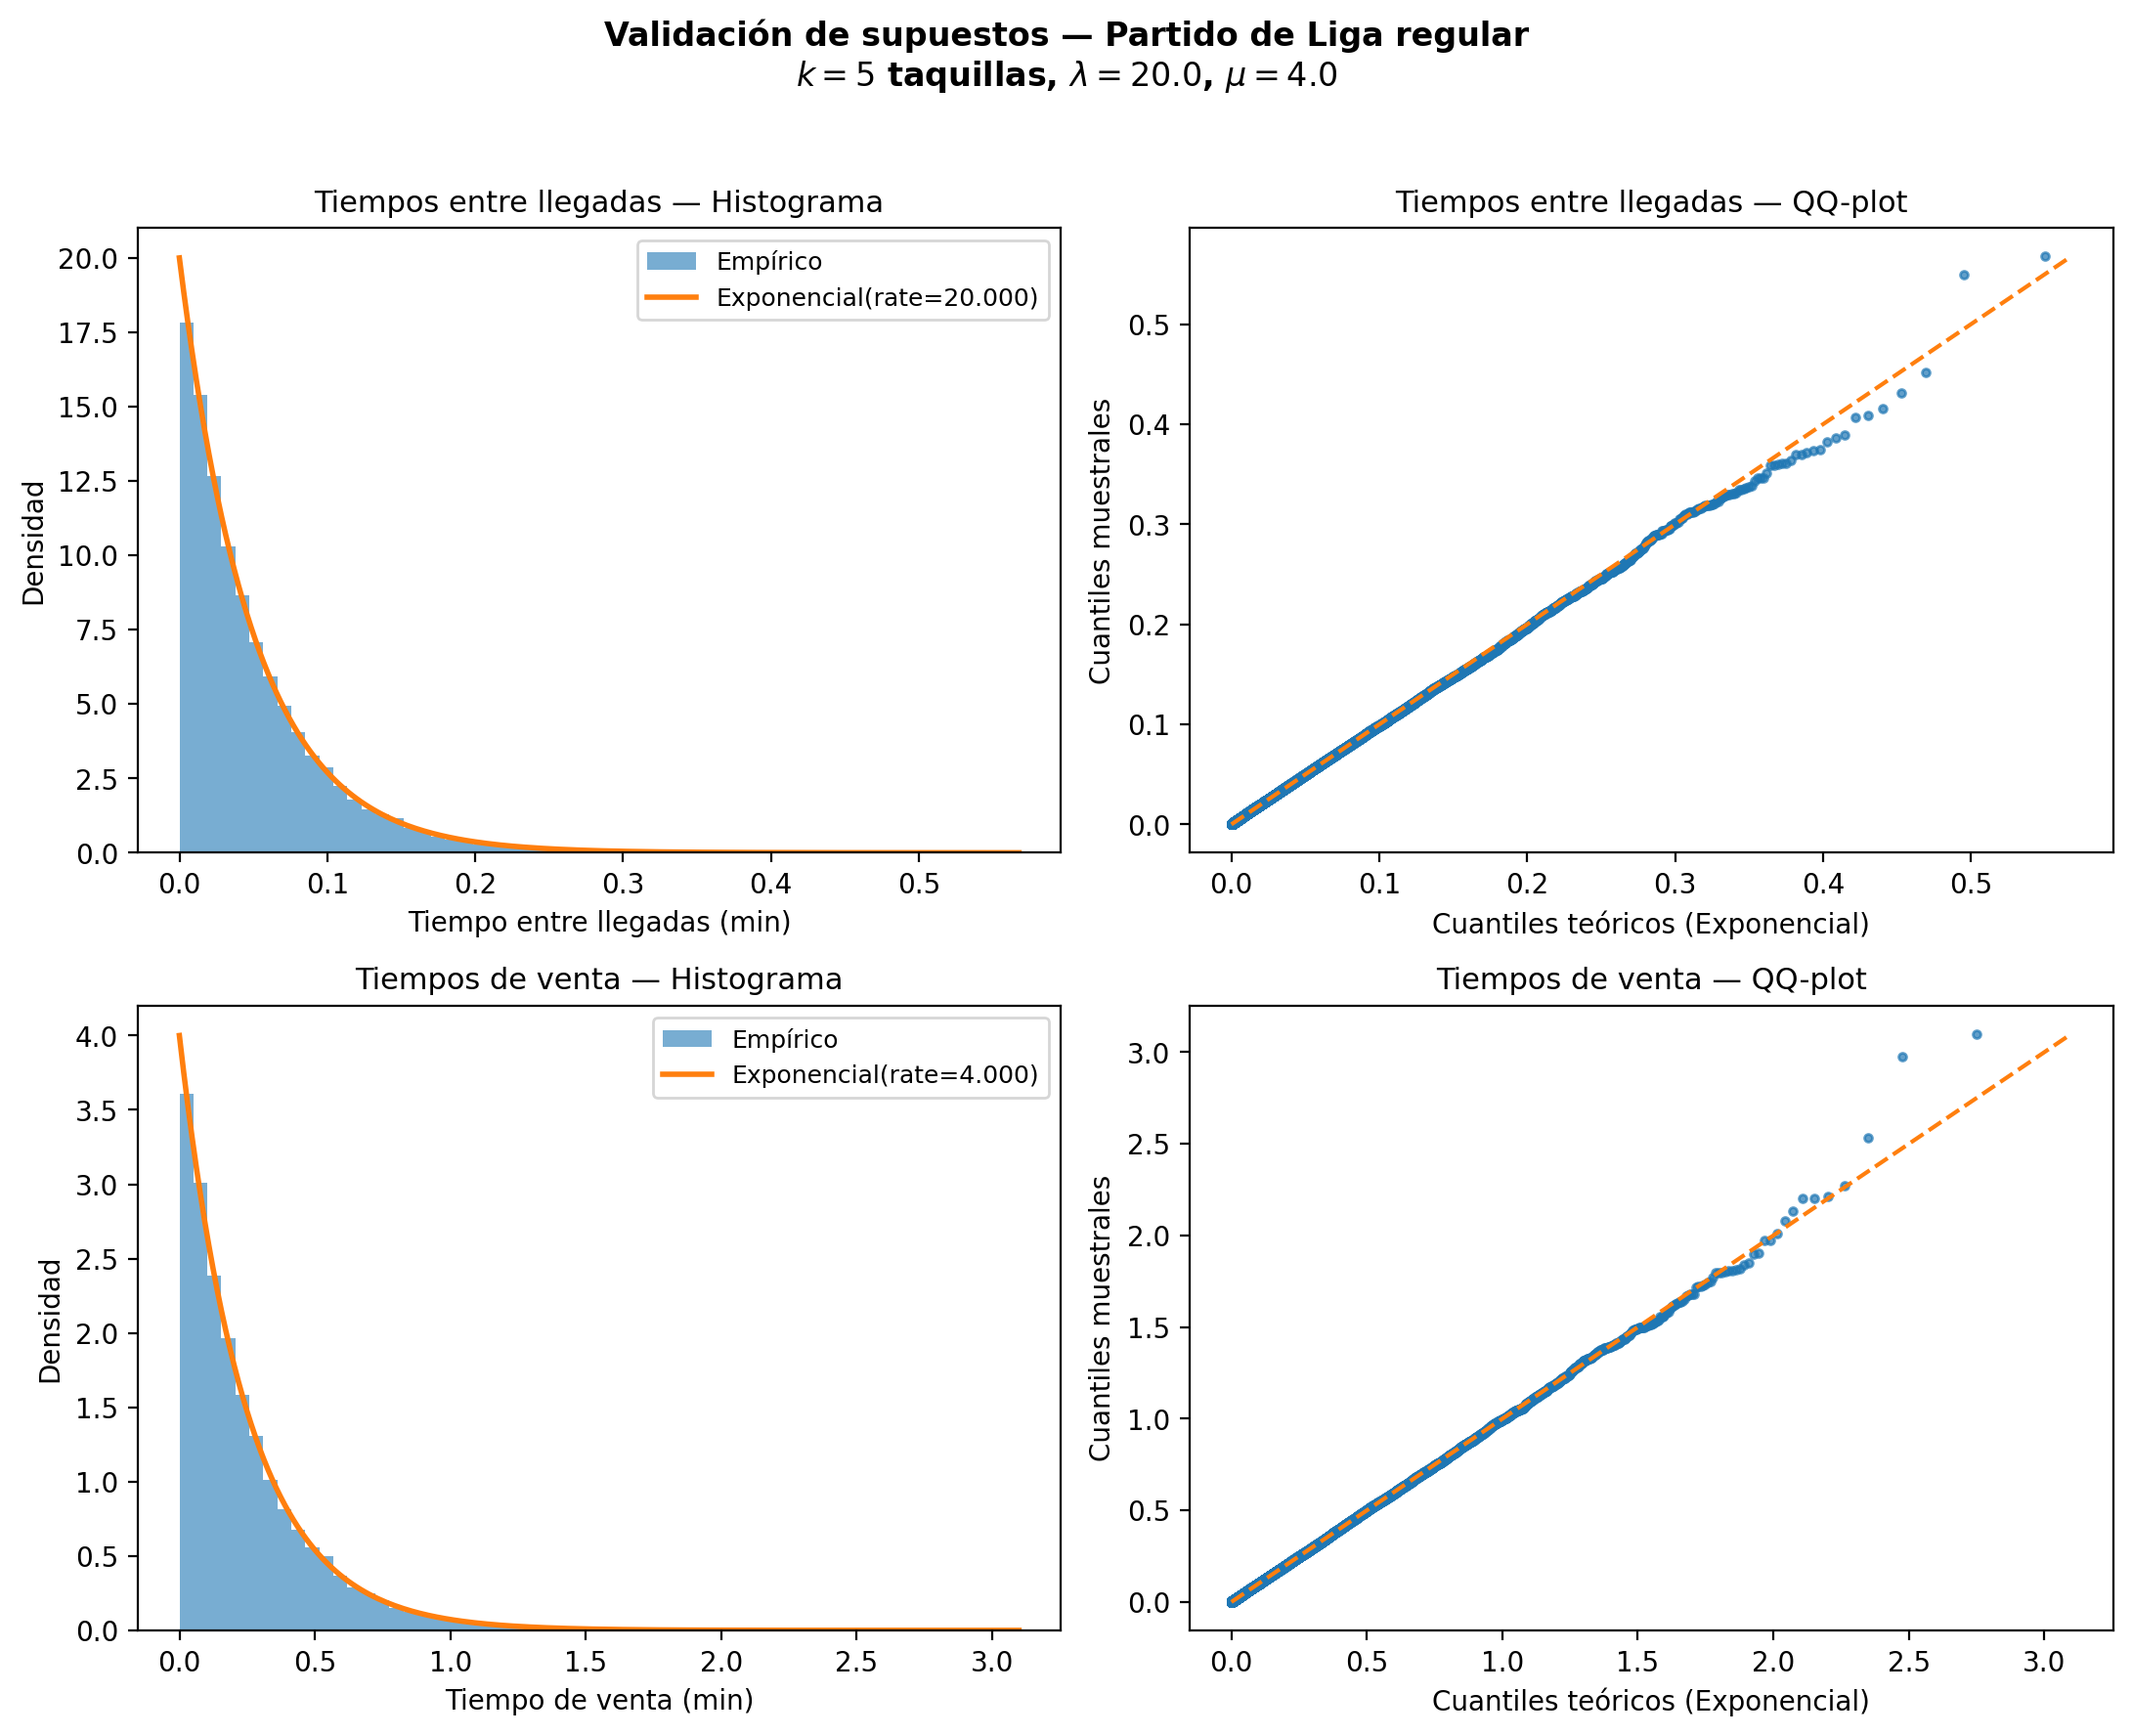
\includegraphics[width=\textwidth]{plots/act_6_santafe/validacion_liga_regular.png}
    \caption{Validación: Liga regular}
\end{subfigure}
\hfill
\begin{subfigure}{0.48\textwidth}
    \centering
    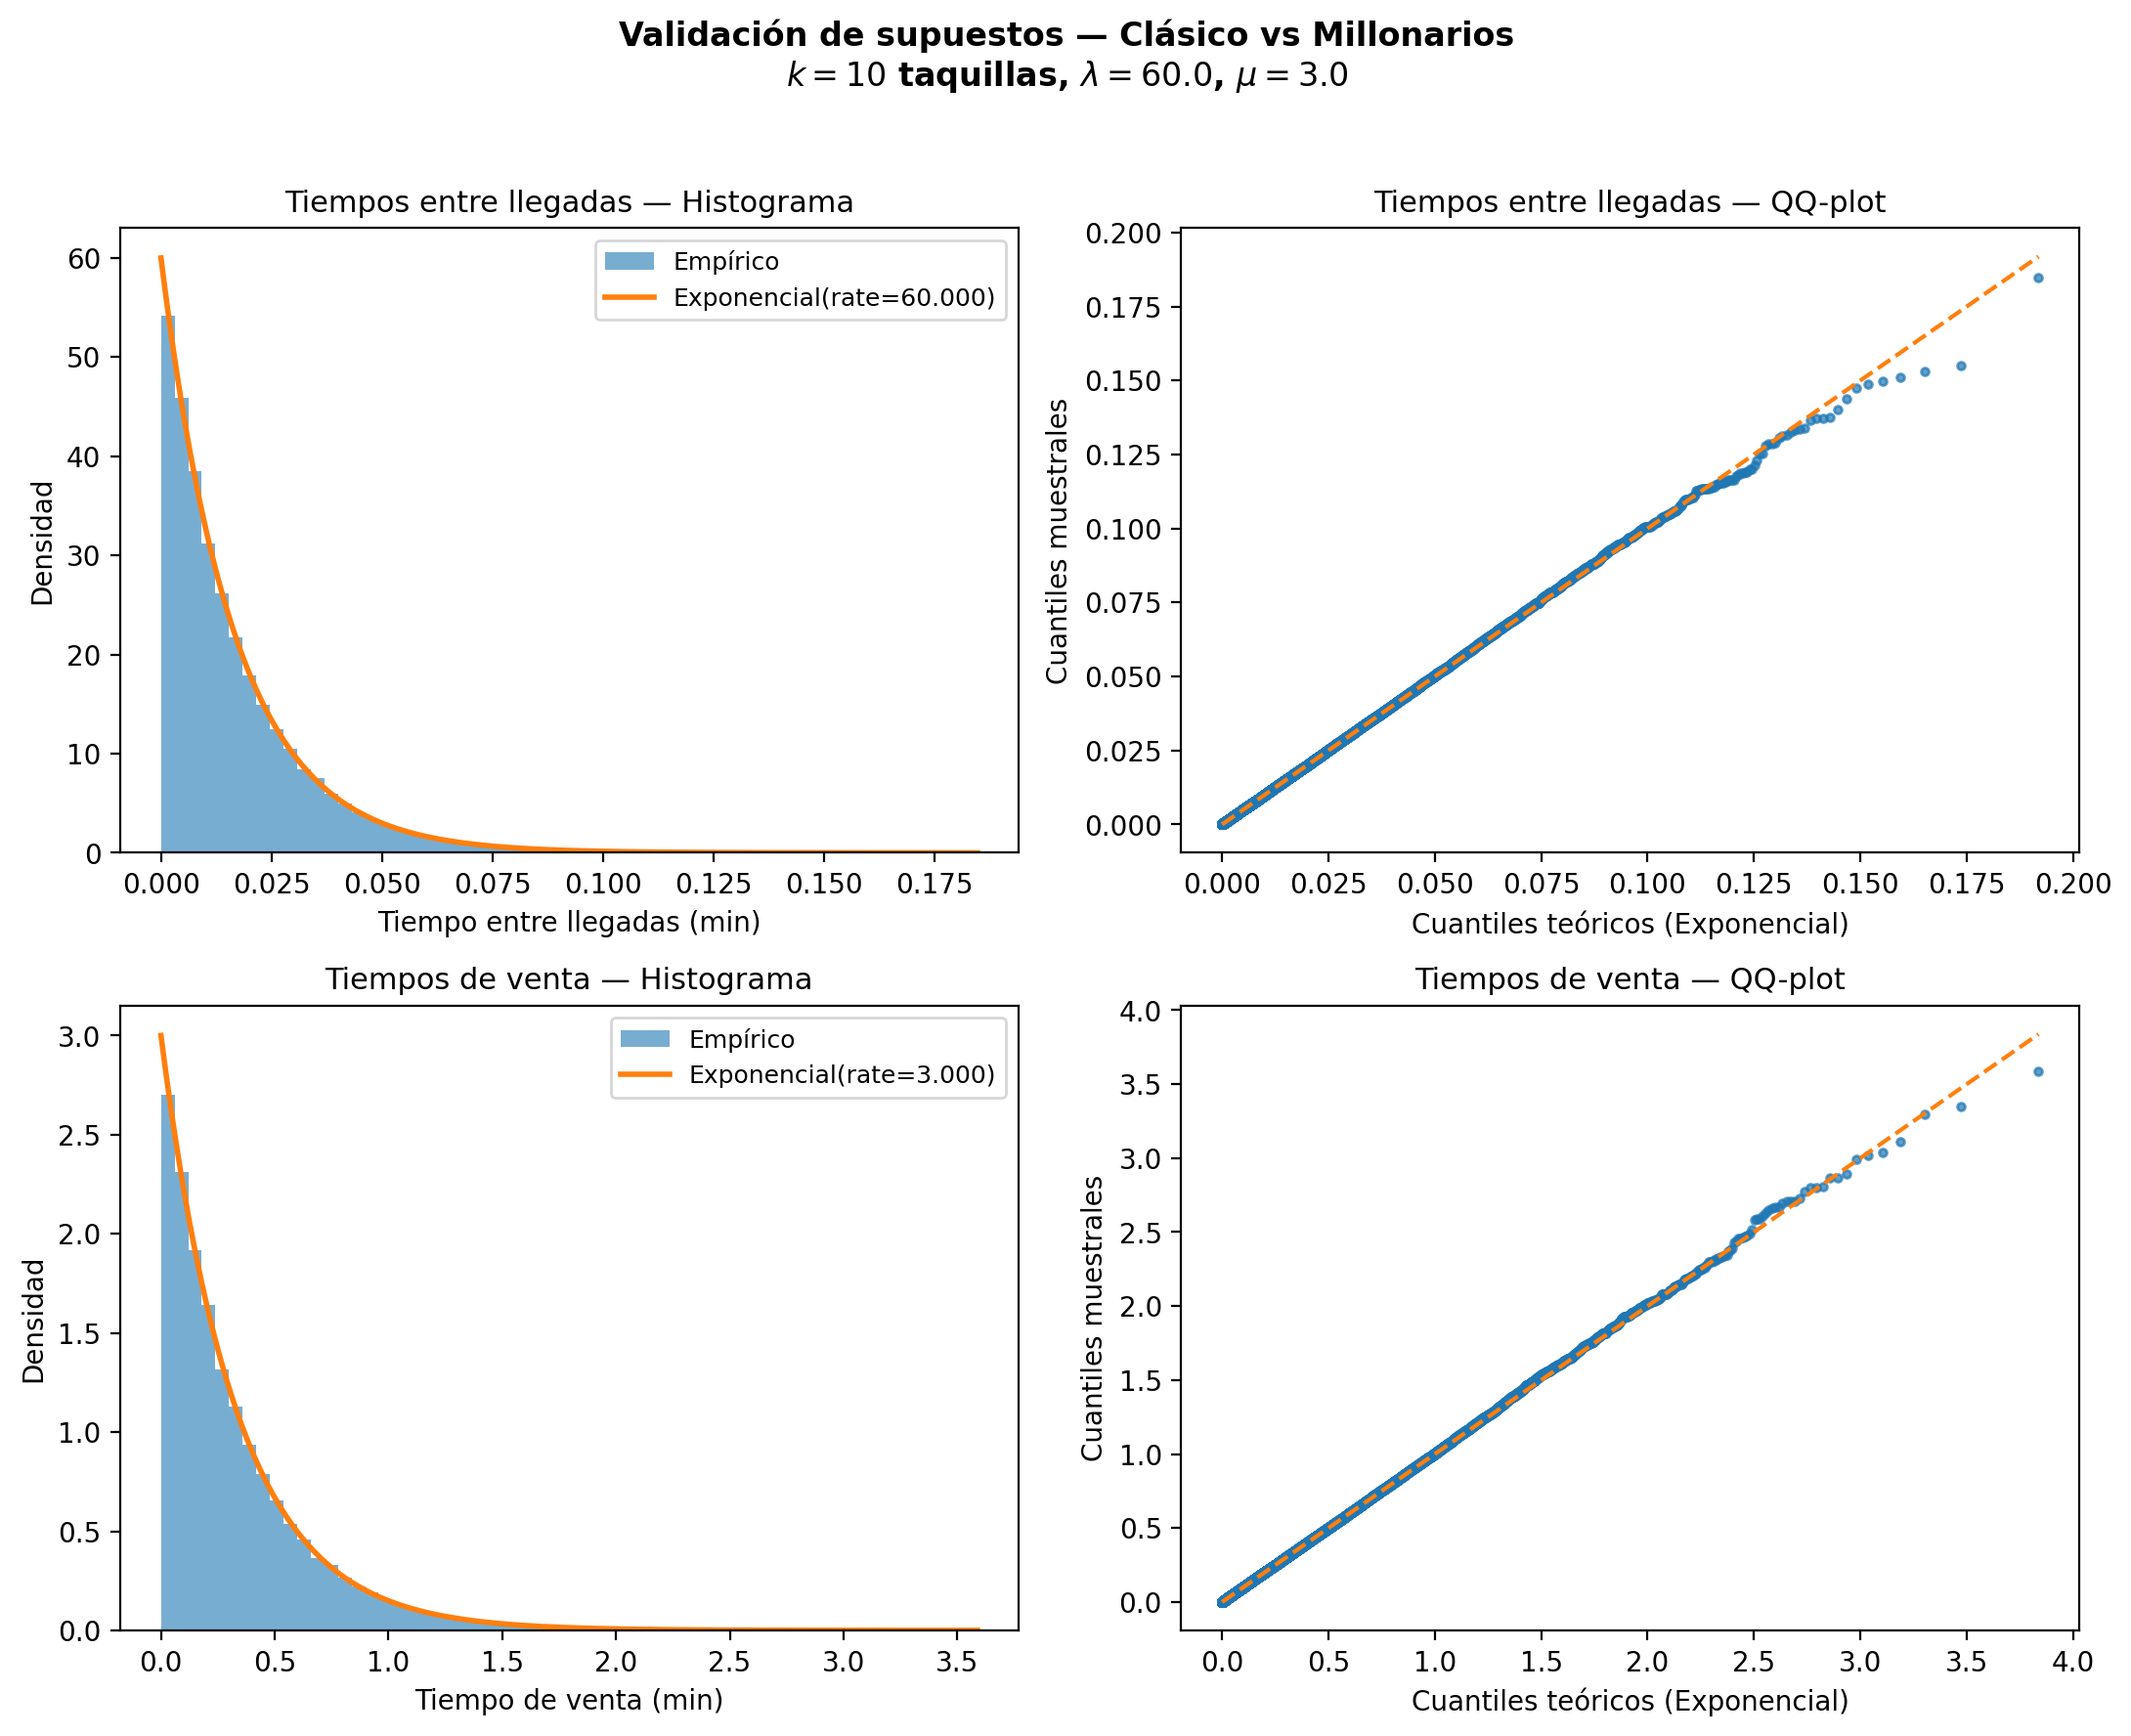
\includegraphics[width=\textwidth]{plots/act_6_santafe/validacion_clasico_millonarios.png}
    \caption{Validación: Clásico Millonarios}
\end{subfigure}
\vspace{1em}
\begin{subfigure}{0.48\textwidth}
    \centering
    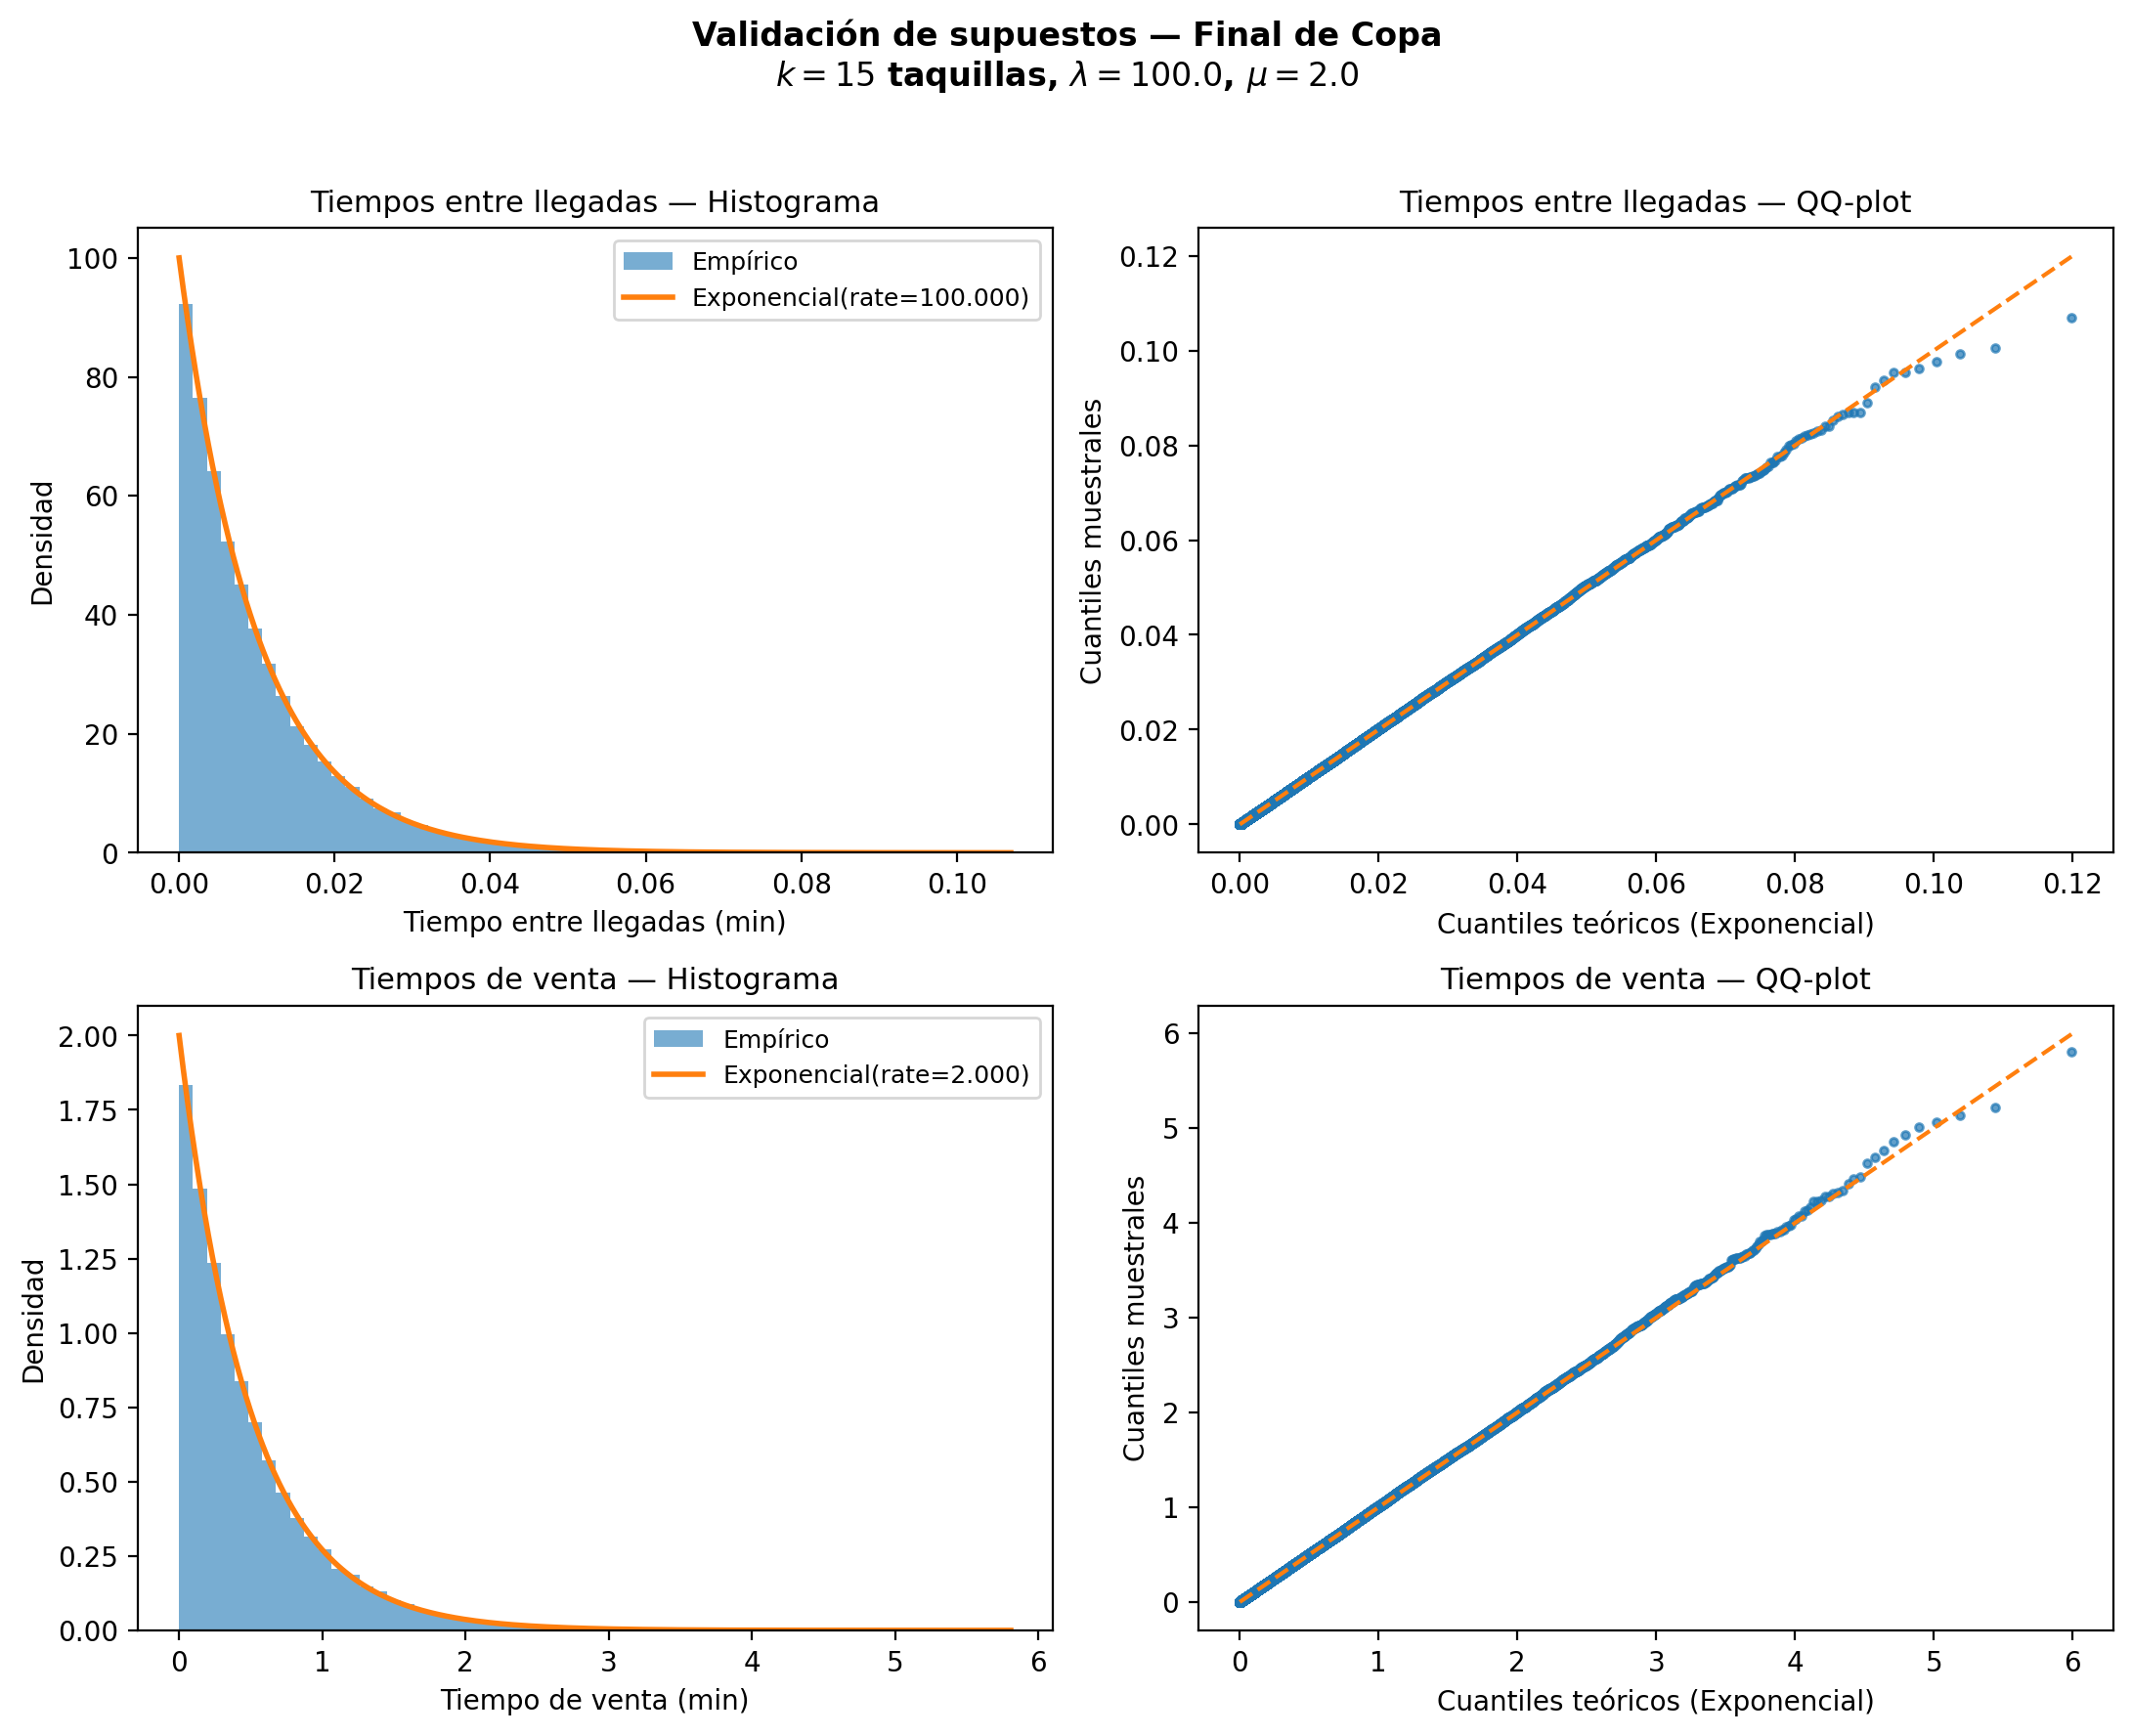
\includegraphics[width=\textwidth]{plots/act_6_santafe/validacion_final_copa.png}
    \caption{Validación: Final de Copa}
\end{subfigure}
\hfill
\begin{subfigure}{0.48\textwidth}
    \centering
    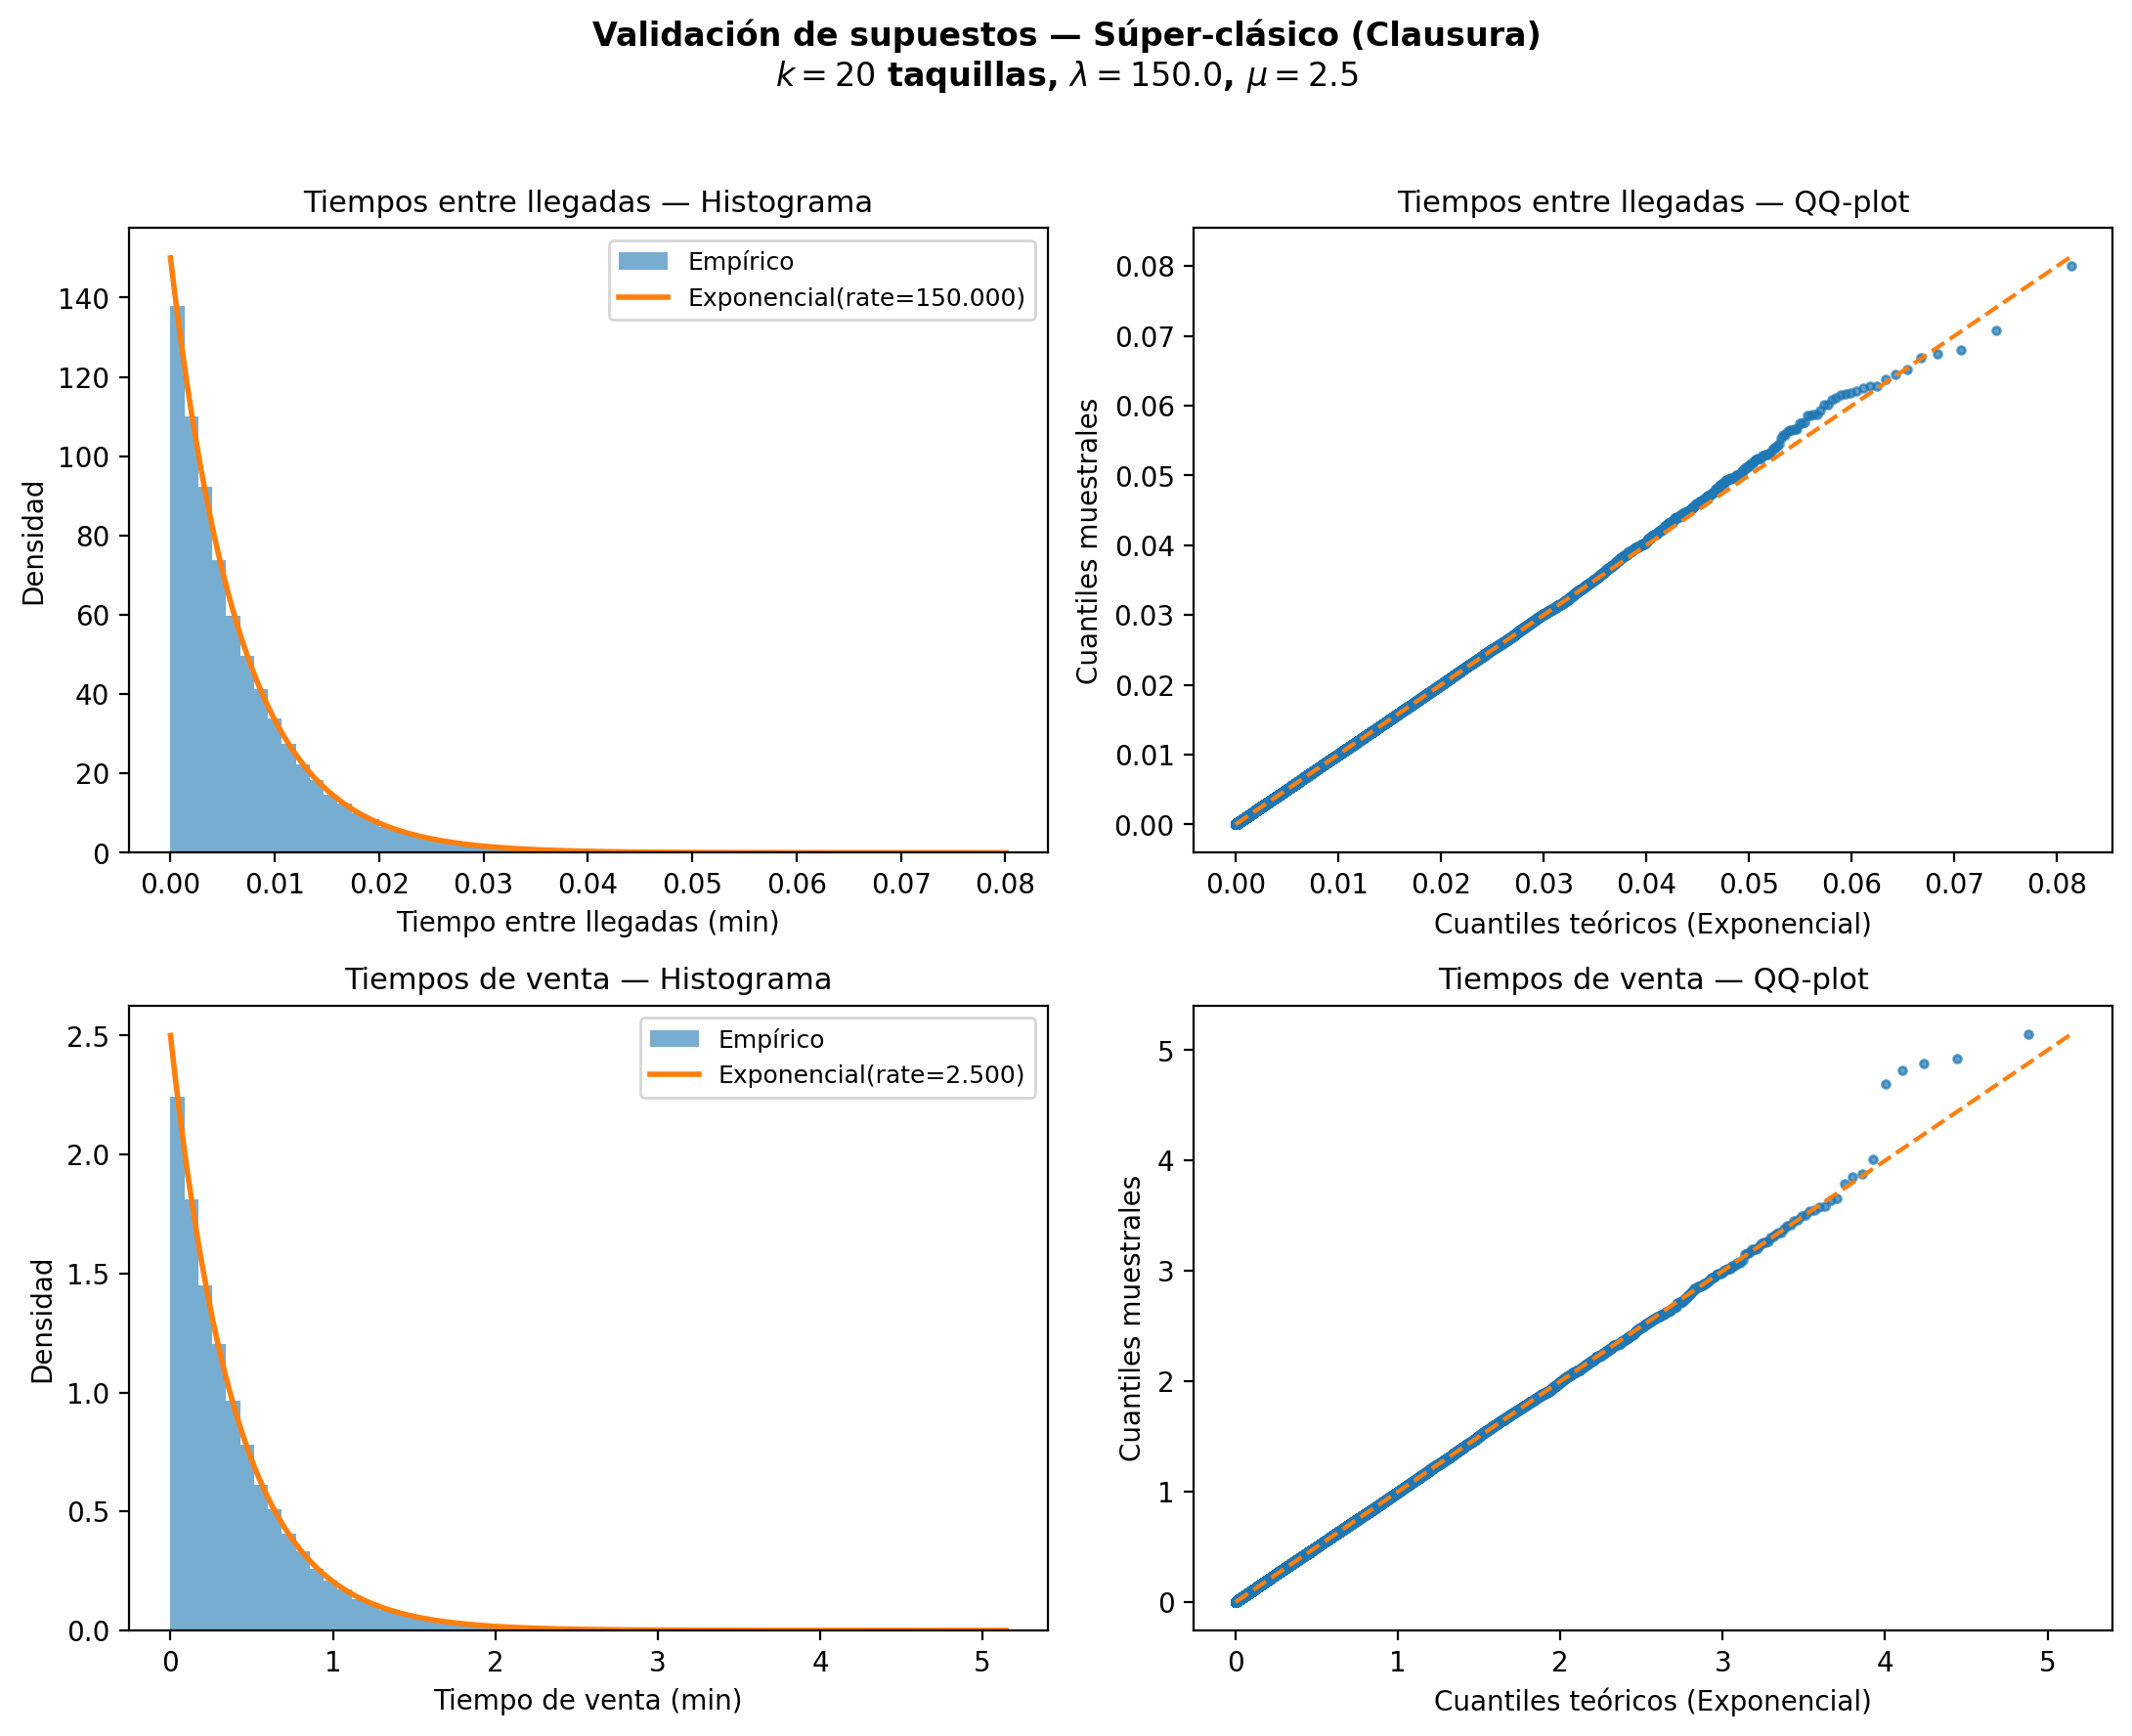
\includegraphics[width=\textwidth]{plots/act_6_santafe/validacion_superclasico.png}
    \caption{Validación: Súper-clásico}
\end{subfigure}
\caption{Análisis de distribución (PDF, CDF, QQ-plot) para los escenarios de venta de
entradas Santa Fe en \emph{Tu Boleta}. Cada figura compara los datos sintéticos con la
distribución exponencial teórica, siguiendo la metodología de las Actividades~4 y~5.}
\label{fig:validacion_tuboleta}
\end{figure}

\subsection*{Simulación y comparación con la teoría}

Se ejecutó un simulador de eventos discretos (SED)~\cite{law2015} (función \texttt{mmkk.m} del curso)
para cada escenario, comparando la probabilidad de bloqueo simulada $\hat{B}$
con el valor teórico $B(k,a)$ de Erlang~B.

\begin{table}[H]
\centering
\caption{Resultados de simulación vs teoría para venta de entradas Santa Fe.}
\label{tab:resultados_tuboleta}
\begin{tabular}{lcccc}
\toprule
\textbf{Escenario} & $B(k,a)$ teórico & $\hat{B}$ simulado & Diferencia & $\rho$ \\
\midrule
Partido de Liga regular & 0.2849 & 0.2857 & 0.0008 & 0.7151 \\
Clásico vs Millonarios & 0.5380 & 0.5365 & 0.0015 & 0.9241 \\
Final de Copa & 0.7080 & 0.7069 & 0.0011 & 0.9735 \\
Súper-clásico (Clausura) & 0.6744 & 0.6783 & 0.0039 & 0.9767 \\
\bottomrule
\end{tabular}
\end{table}

\begin{remark}
La diferencia entre teoría y simulación es menor al $0.01$ en todos los casos,
validando tanto la implementación del simulador como la aplicabilidad del modelo
M/M/k/k al caso real de una plataforma de venta de entradas para fútbol.
\end{remark}

\begin{figure}[H]
\centering
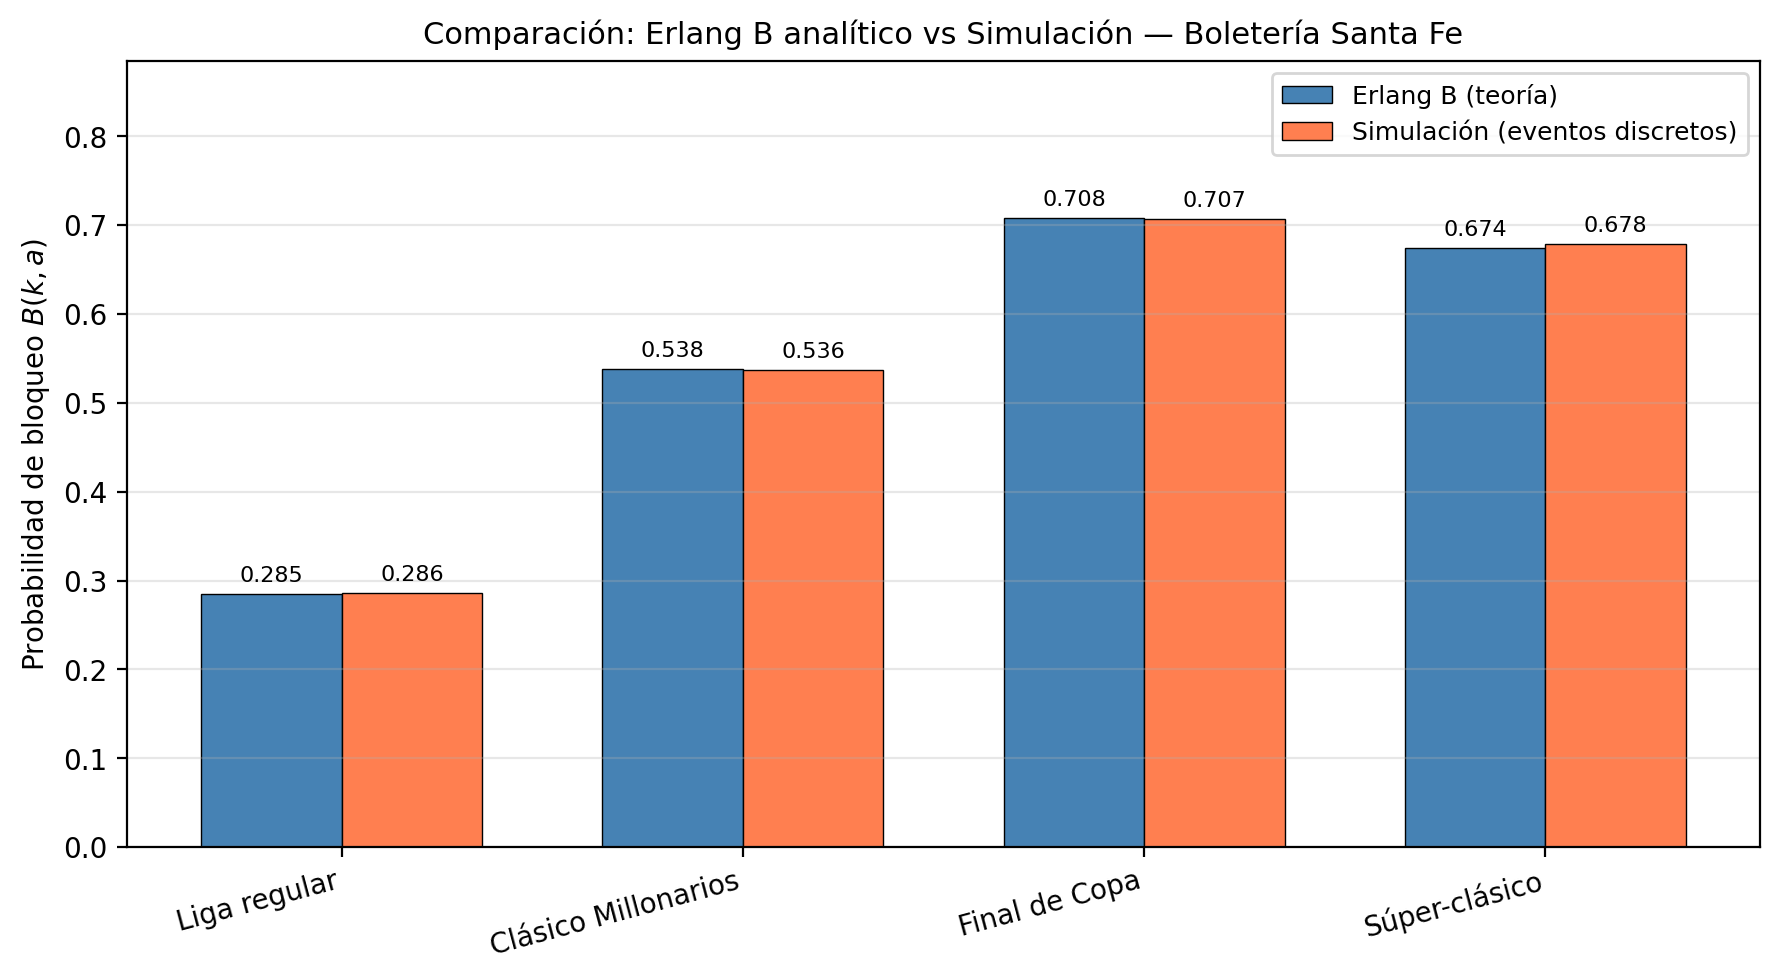
\includegraphics[width=0.95\textwidth]{plots/act_6_santafe/comparacion_bloqueo.png}
\caption{Comparación entre Erlang~B analítico y simulación por eventos discretos
para los escenarios de venta de entradas Santa Fe en \emph{Tu Boleta}.}
\label{fig:comparacion_tuboleta}
\end{figure}

\subsection*{Curvas de sensibilidad y punto de operación}

La Figura~\ref{fig:curvas_tuboleta} muestra cómo crece la probabilidad de bloqueo
al aumentar la tasa de llegadas $\lambda$, manteniendo fijos $k$ y $\mu$ en cada
escenario. Se destaca el punto de operación actual y la línea de referencia
$B_{\max}=0.05$.

\begin{figure}[H]
\centering
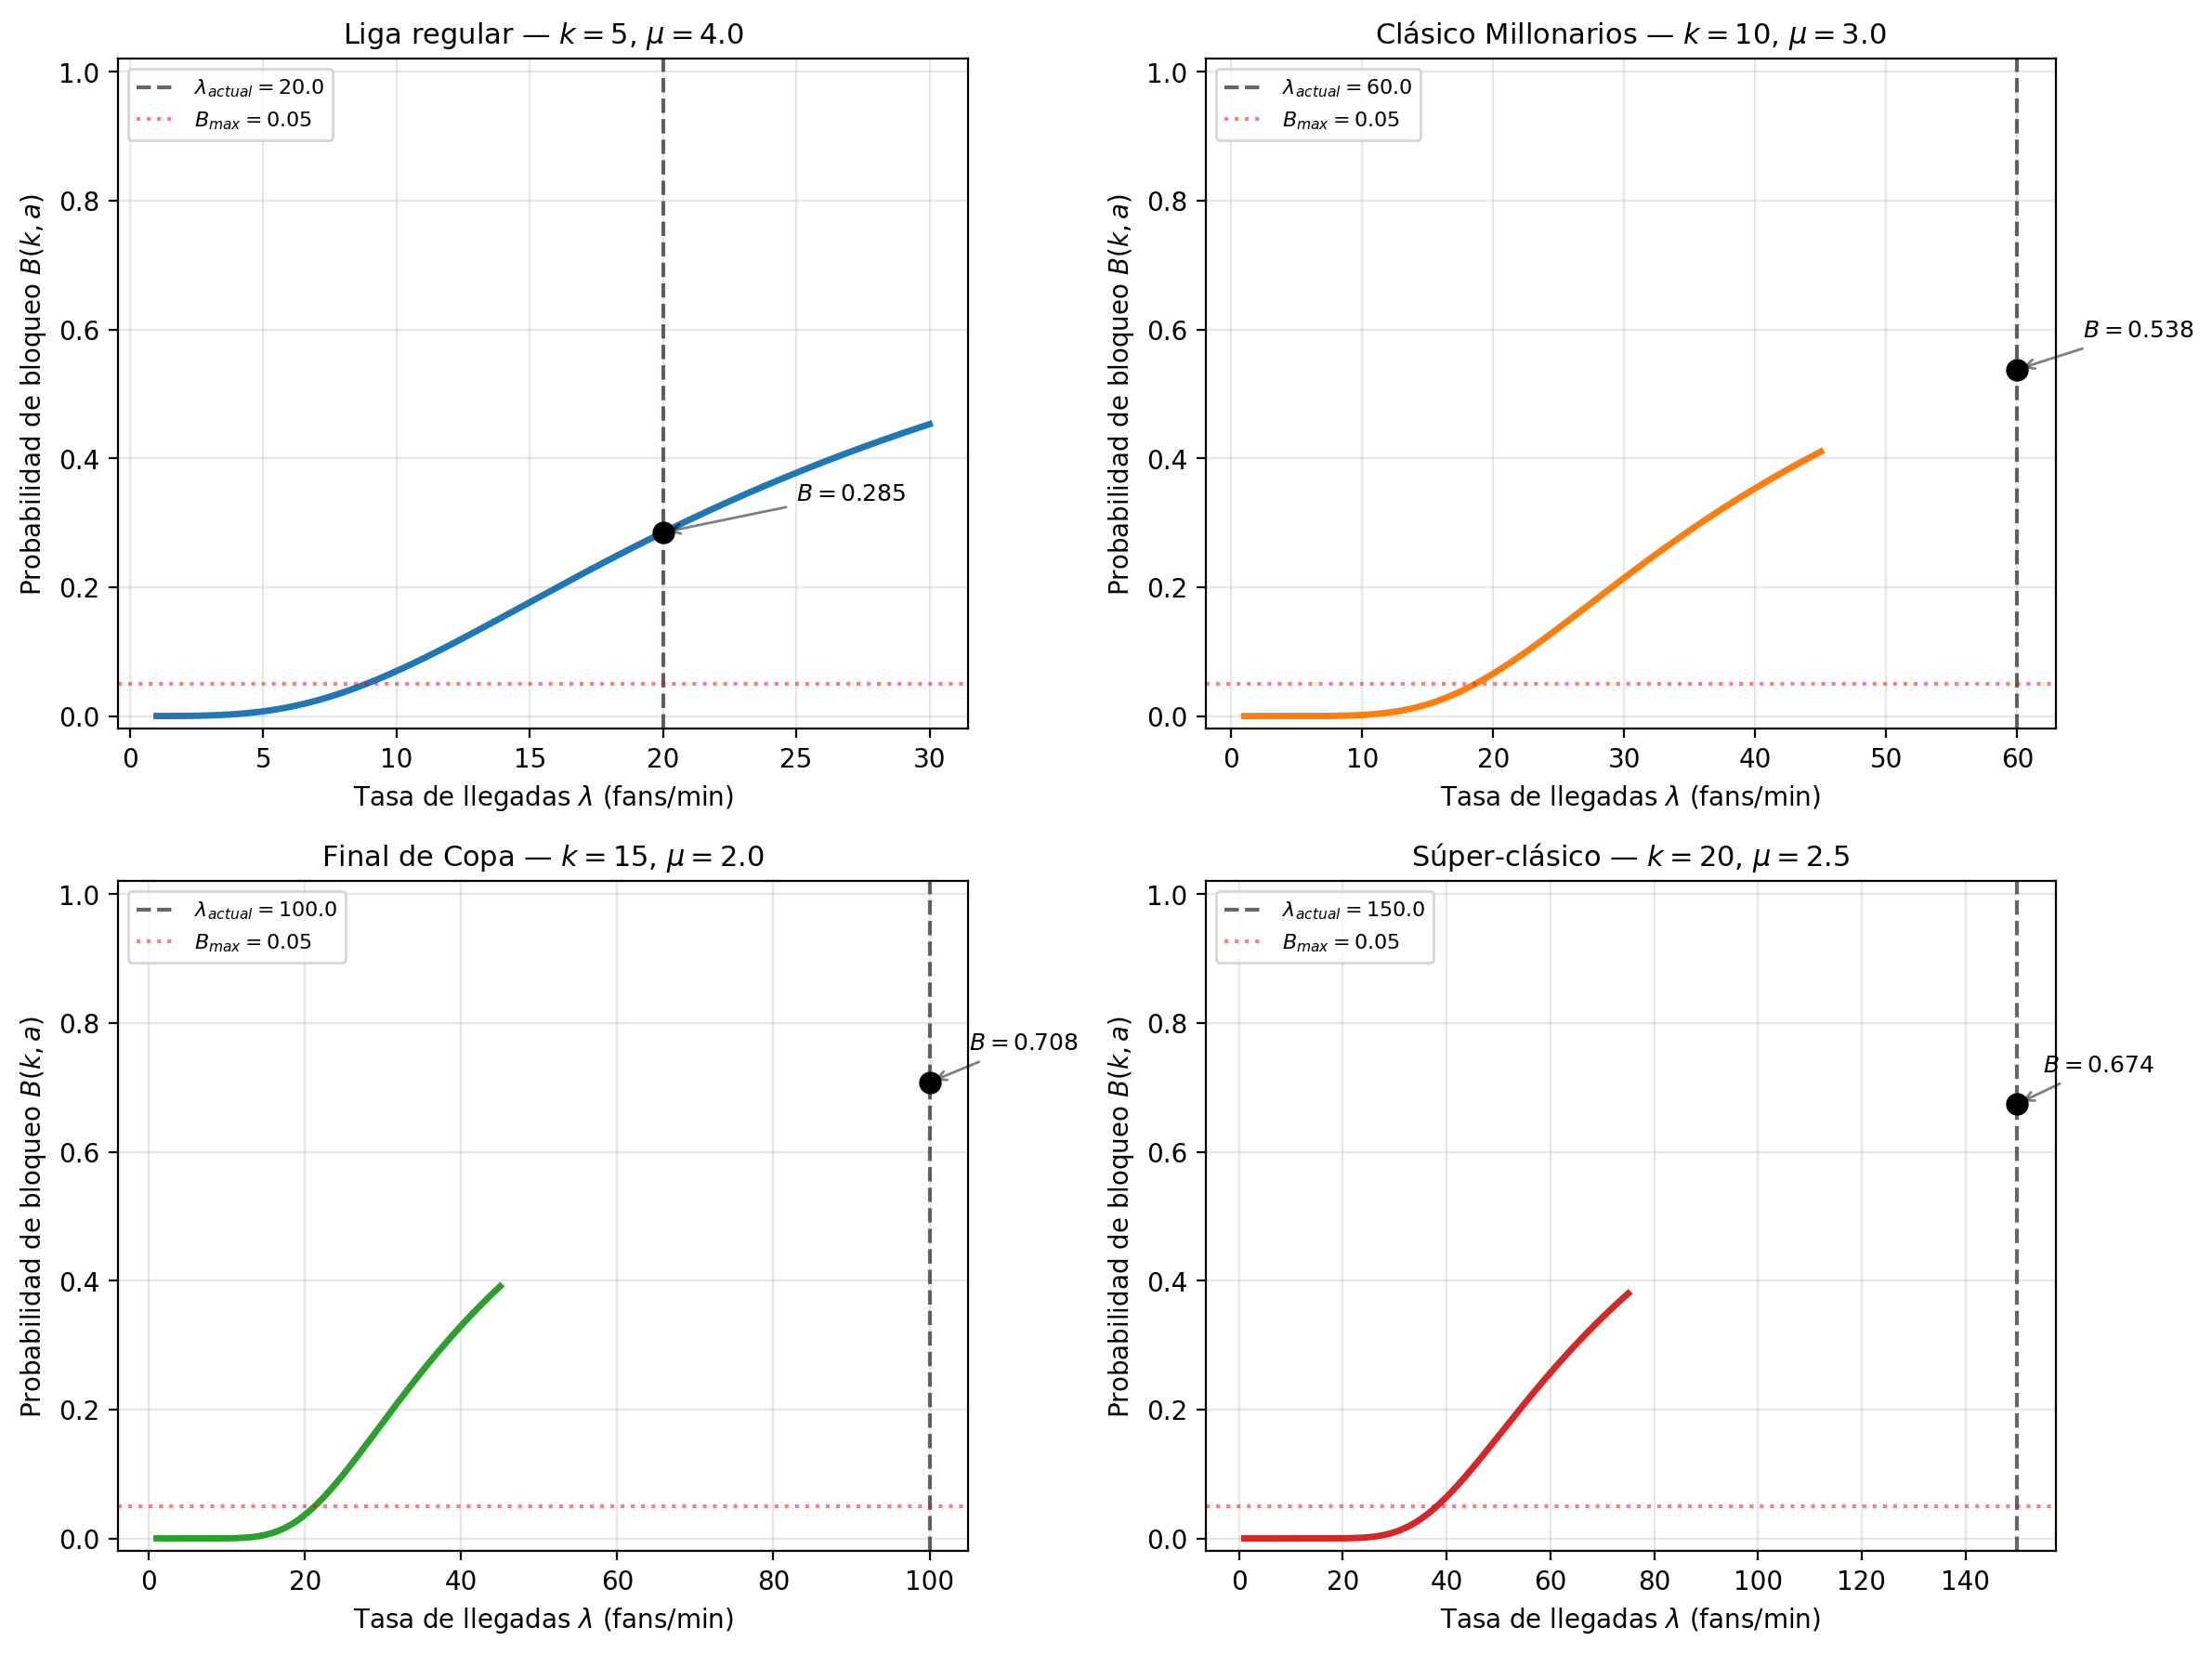
\includegraphics[width=0.98\textwidth]{plots/act_6_santafe/curvas_erlang_por_escenario.png}
\caption{Curvas de Erlang~B para cada escenario de venta de entradas Santa Fe.
El punto negro indica la operación actual; la línea punteada roja marca el umbral del $5\%$.}
\label{fig:curvas_tuboleta}
\end{figure}

\subsection*{Evolución temporal de la ocupación}

La Figura~\ref{fig:ocupacion_tuboleta} muestra la evolución temporal del número de
instancias ocupadas en una ventana de 30 minutos. En los escenarios de alta demanda
(Final y Súper-clásico) las instancias permanecen casi permanentemente saturadas.

\begin{figure}[H]
\centering
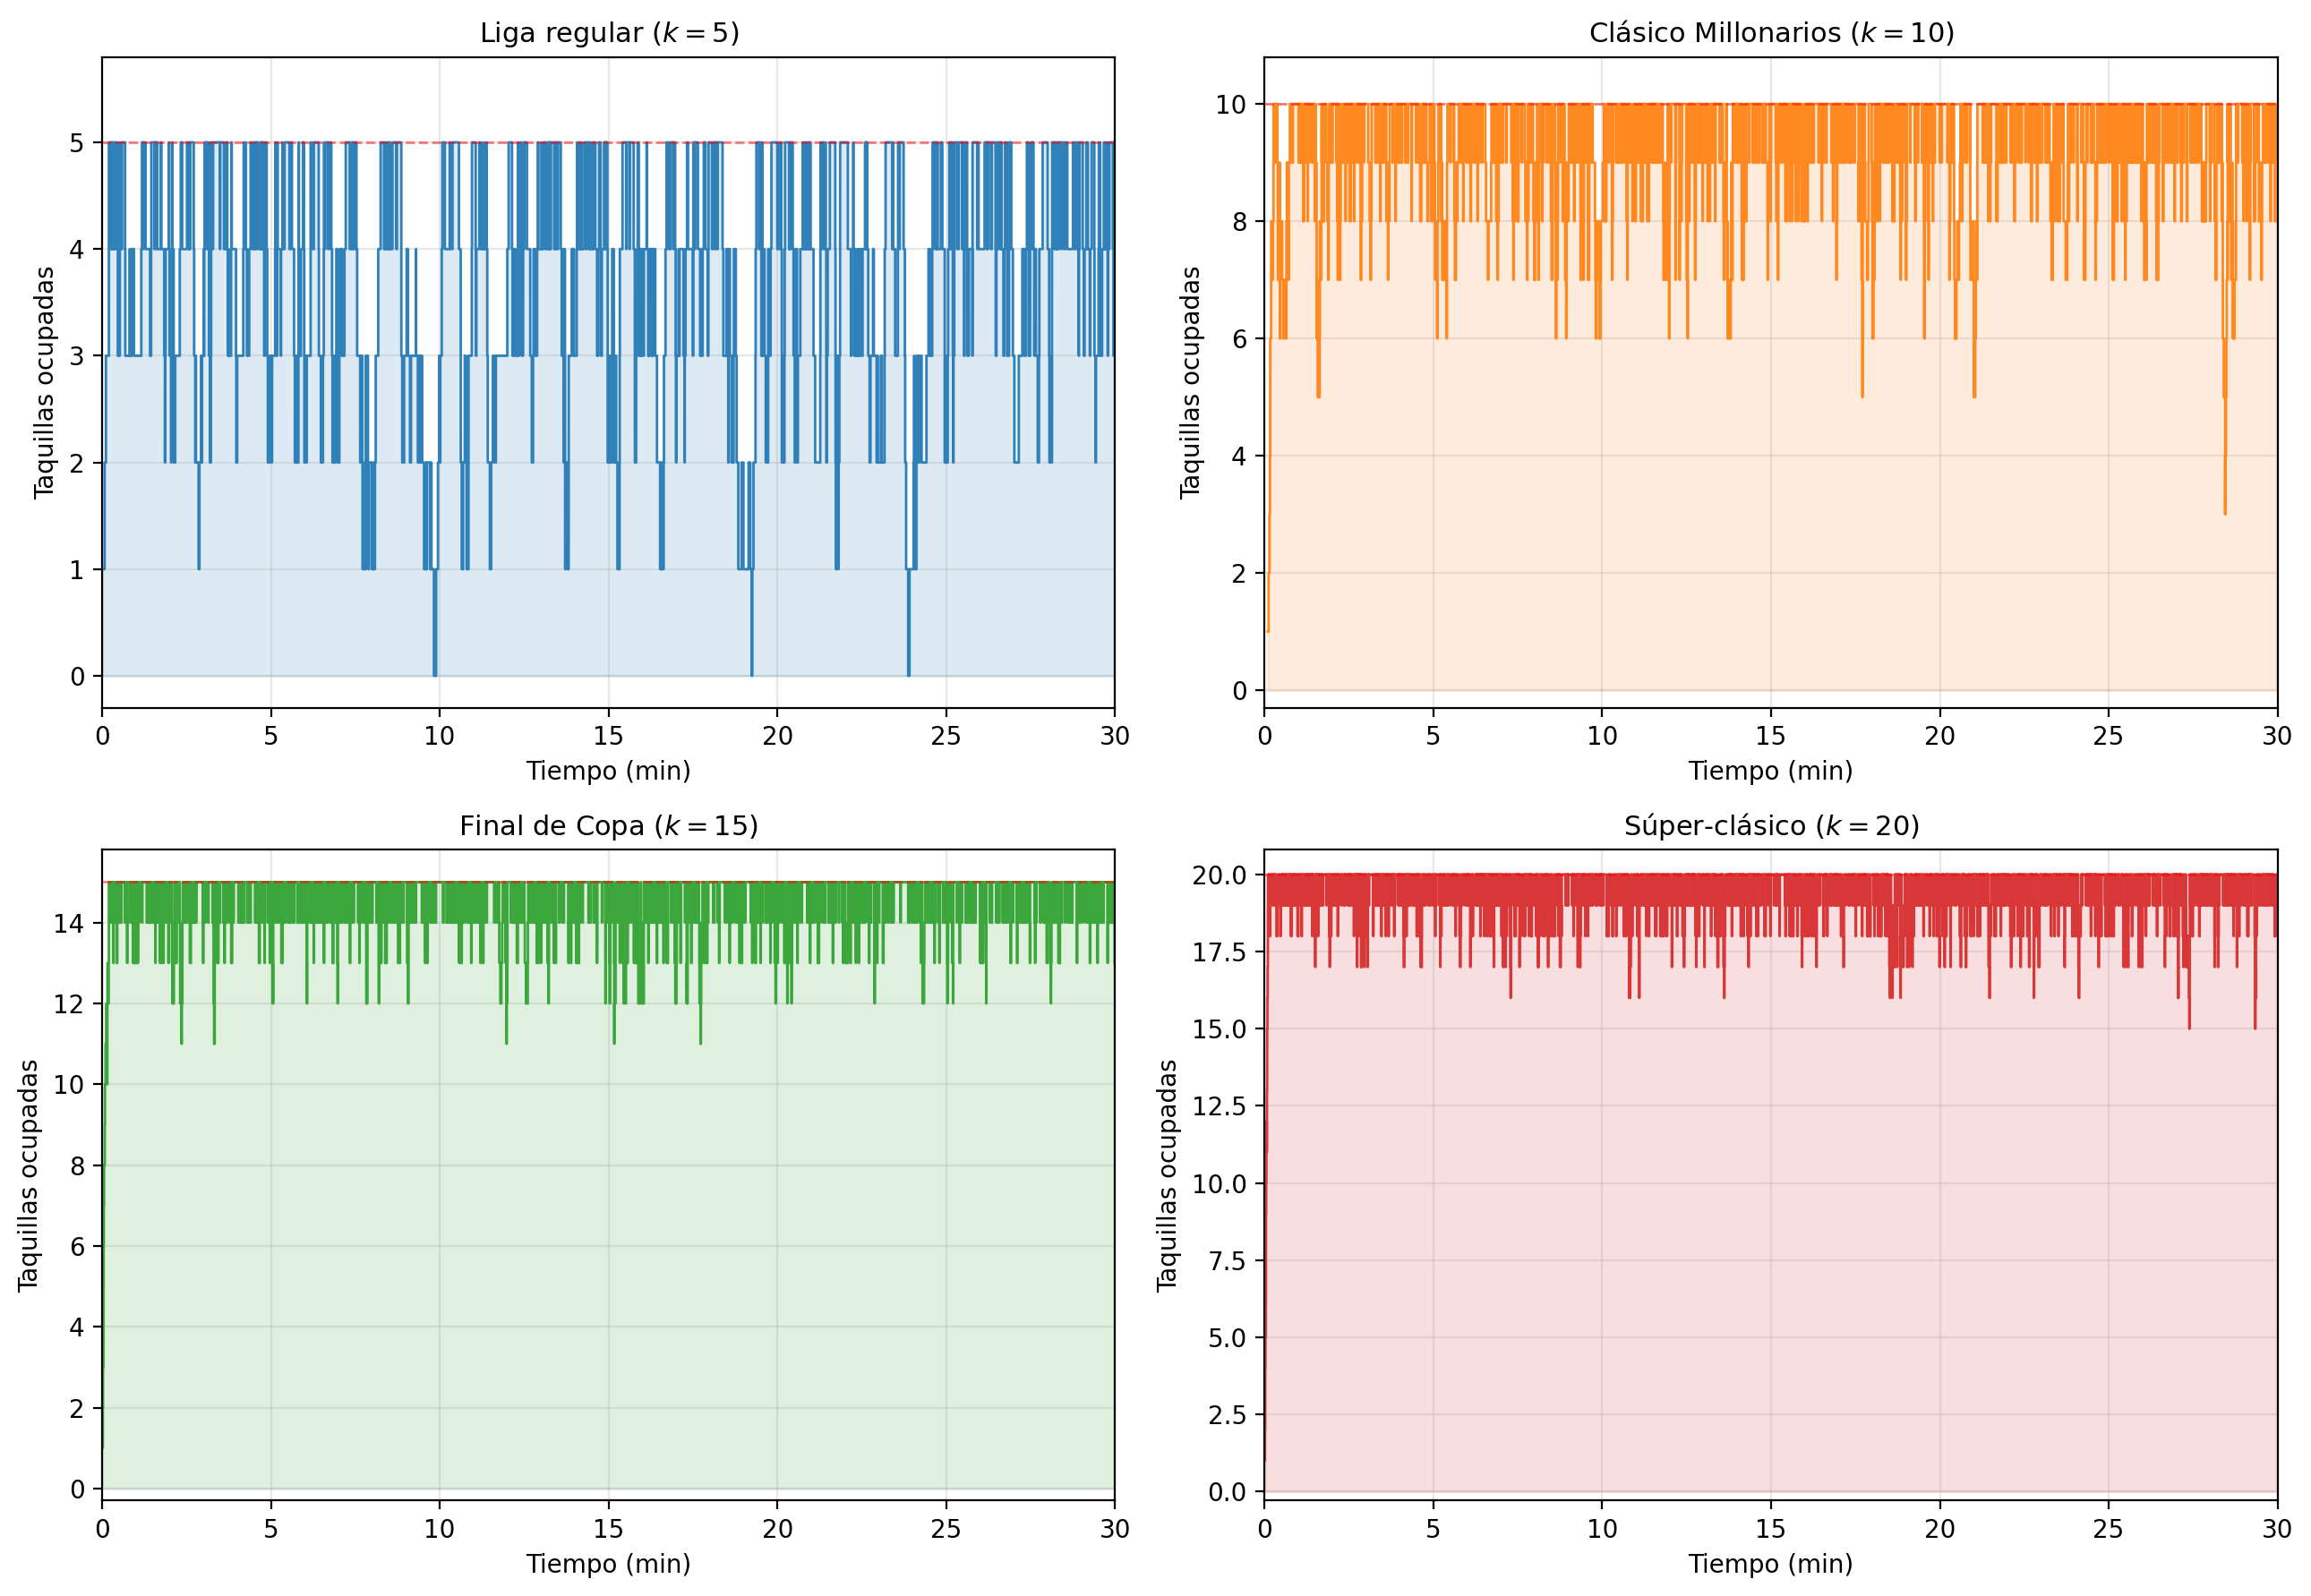
\includegraphics[width=0.98\textwidth]{plots/act_6_santafe/ocupacion_temporal_todos.png}
\caption{Evolución temporal de la ocupación de instancias en los primeros 30 minutos
de venta para cada escenario. La línea roja punteada indica la capacidad máxima $k$.}
\label{fig:ocupacion_tuboleta}
\end{figure}

\subsection*{Dimensionamiento óptimo del servidor}

La Tabla~\ref{tab:dimensionamiento_tuboleta} presenta el número mínimo de instancias
$k^*$ necesarias para cumplir distintos niveles de calidad de servicio, calculado
mediante la recursión de Jagerman.

\begin{table}[H]
\centering
\caption{Dimensionamiento óptimo de instancias para venta de entradas Santa Fe.}
\label{tab:dimensionamiento_tuboleta}
\begin{tabular}{l|cccc}
\toprule
& \multicolumn{4}{c}{\textbf{$k^*$ mínimo para umbral $B_{\max}$}} \\
\textbf{Escenario} & $0.001$ & $0.01$ & $0.05$ & $0.10$ \\
\midrule
Partido de Liga regular & 14 & 11 & 9 & 8 \\
Clásico vs Millonarios & 35 & 30 & 26 & 23 \\
Final de Copa & 71 & 64 & 56 & 51 \\
Súper-clásico (Clausura) & 83 & 75 & 66 & 60 \\
\bottomrule
\end{tabular}
\end{table}

\begin{figure}[H]
\centering
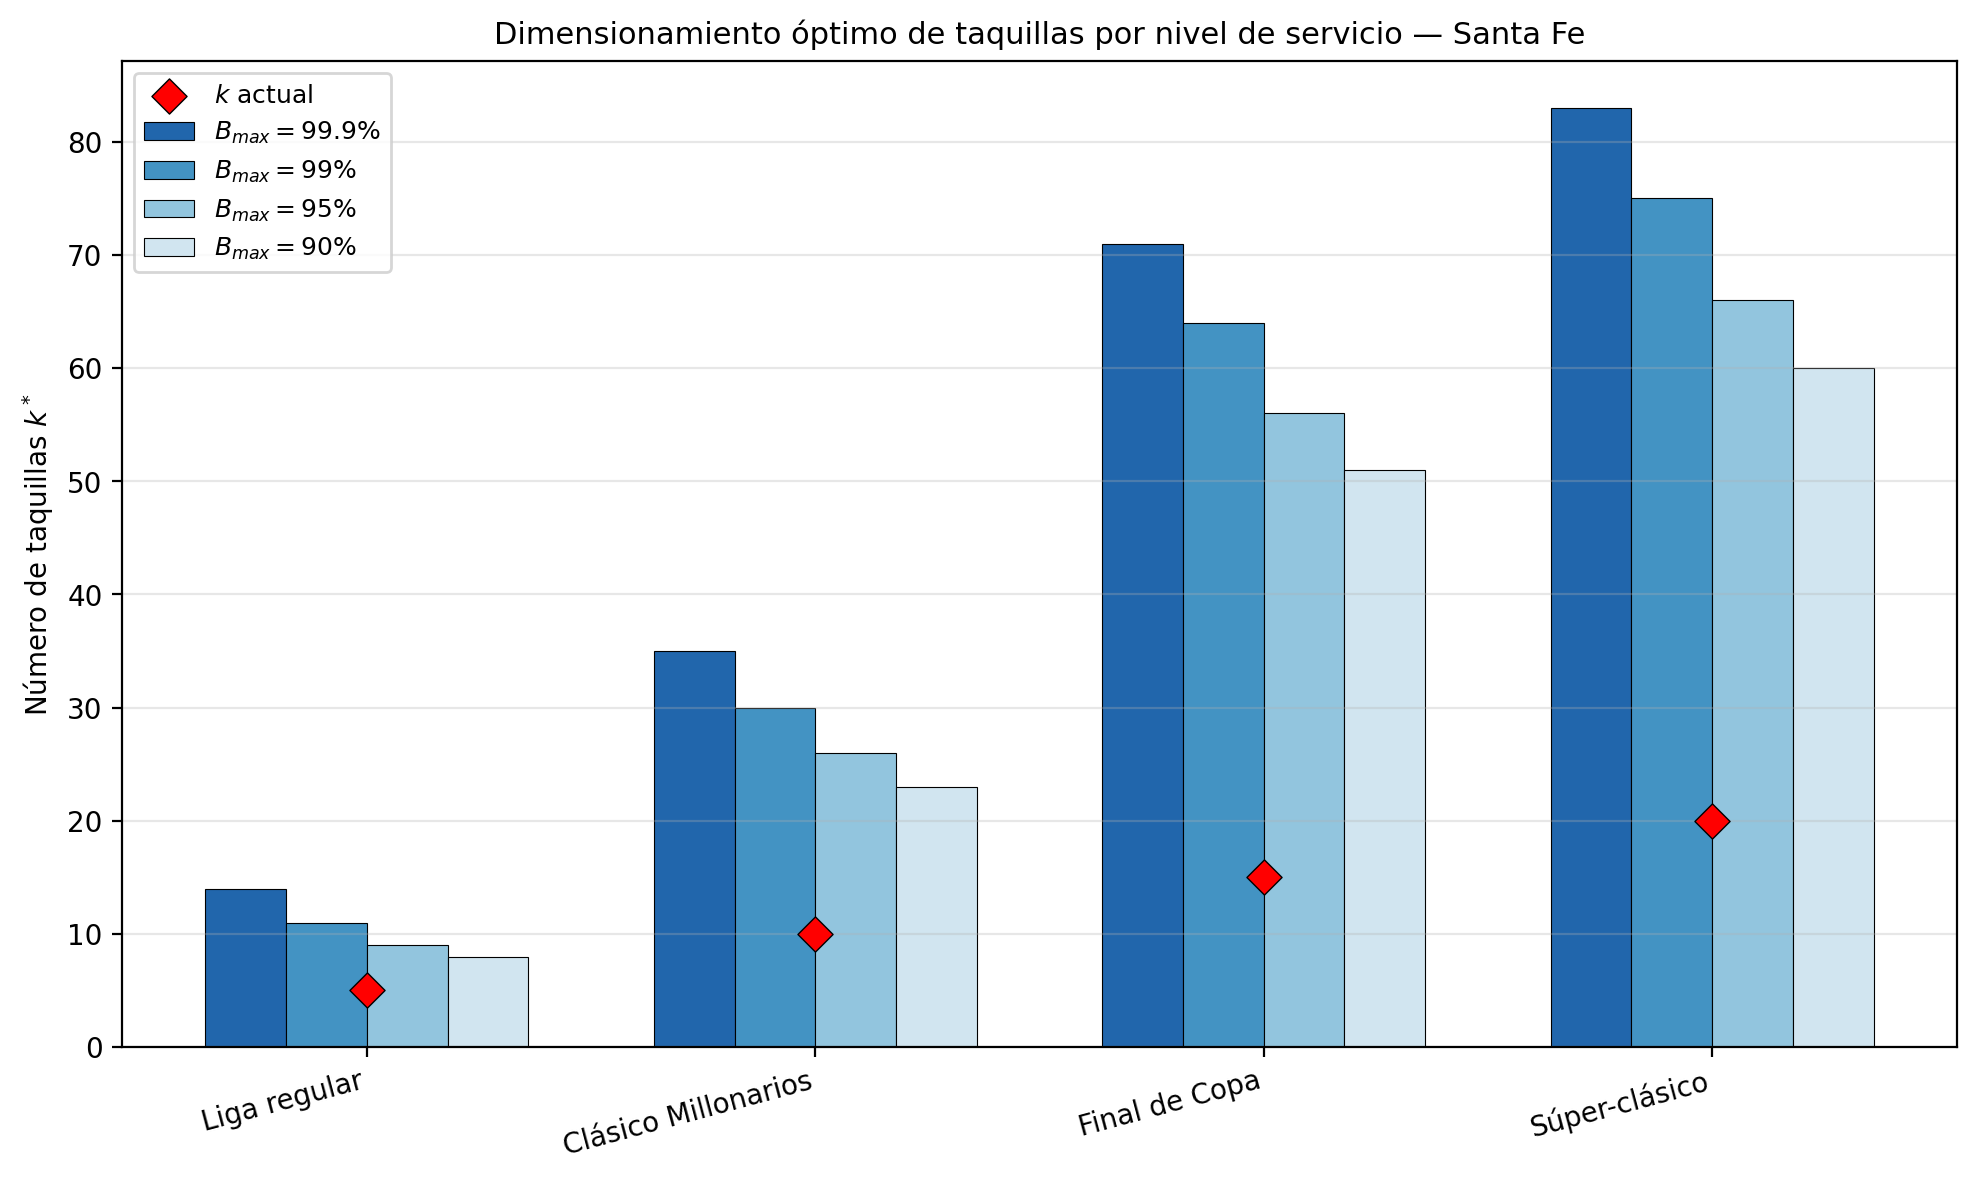
\includegraphics[width=0.95\textwidth]{plots/act_6_santafe/dimensionamiento_optimo.png}
\caption{Dimensionamiento óptimo de instancias por nivel de servicio.
El rombo rojo indica la configuración actual de cada escenario.}
\label{fig:dimensionamiento_tuboleta}
\end{figure}

\begin{remark}
Los resultados muestran que la configuración actual es \emph{insuficiente} para todos
los escenarios. Para el Clásico vs Millonarios, que genera una carga de $a=20$ Erlangs
con solo $k=10$ instancias, el $53.8\%$ de los hinchas que intentan comprar se quedan
sin entrada ($B=0.538$). Para cumplir un nivel de servicio del $95\%$ ($B_{\max}=0.05$),
\emph{Tu Boleta} necesitaría $k^*=26$ instancias ---casi el triple de las actuales.
En el Súper-clásico, la situación es aún más crítica: se requieren $k^*=60$ instancias
para el umbral del $10\%$, frente a las $k=20$ actuales.
\end{remark}

\subsection*{Distribución estacionaria}

La Figura~\ref{fig:distribucion_tuboleta} muestra la distribución estacionaria $P_n$
de probabilidades para cada escenario. La barra roja destaca $P_k$, la probabilidad de
que todas las instancias estén ocupadas (bloqueo).

\begin{figure}[H]
\centering
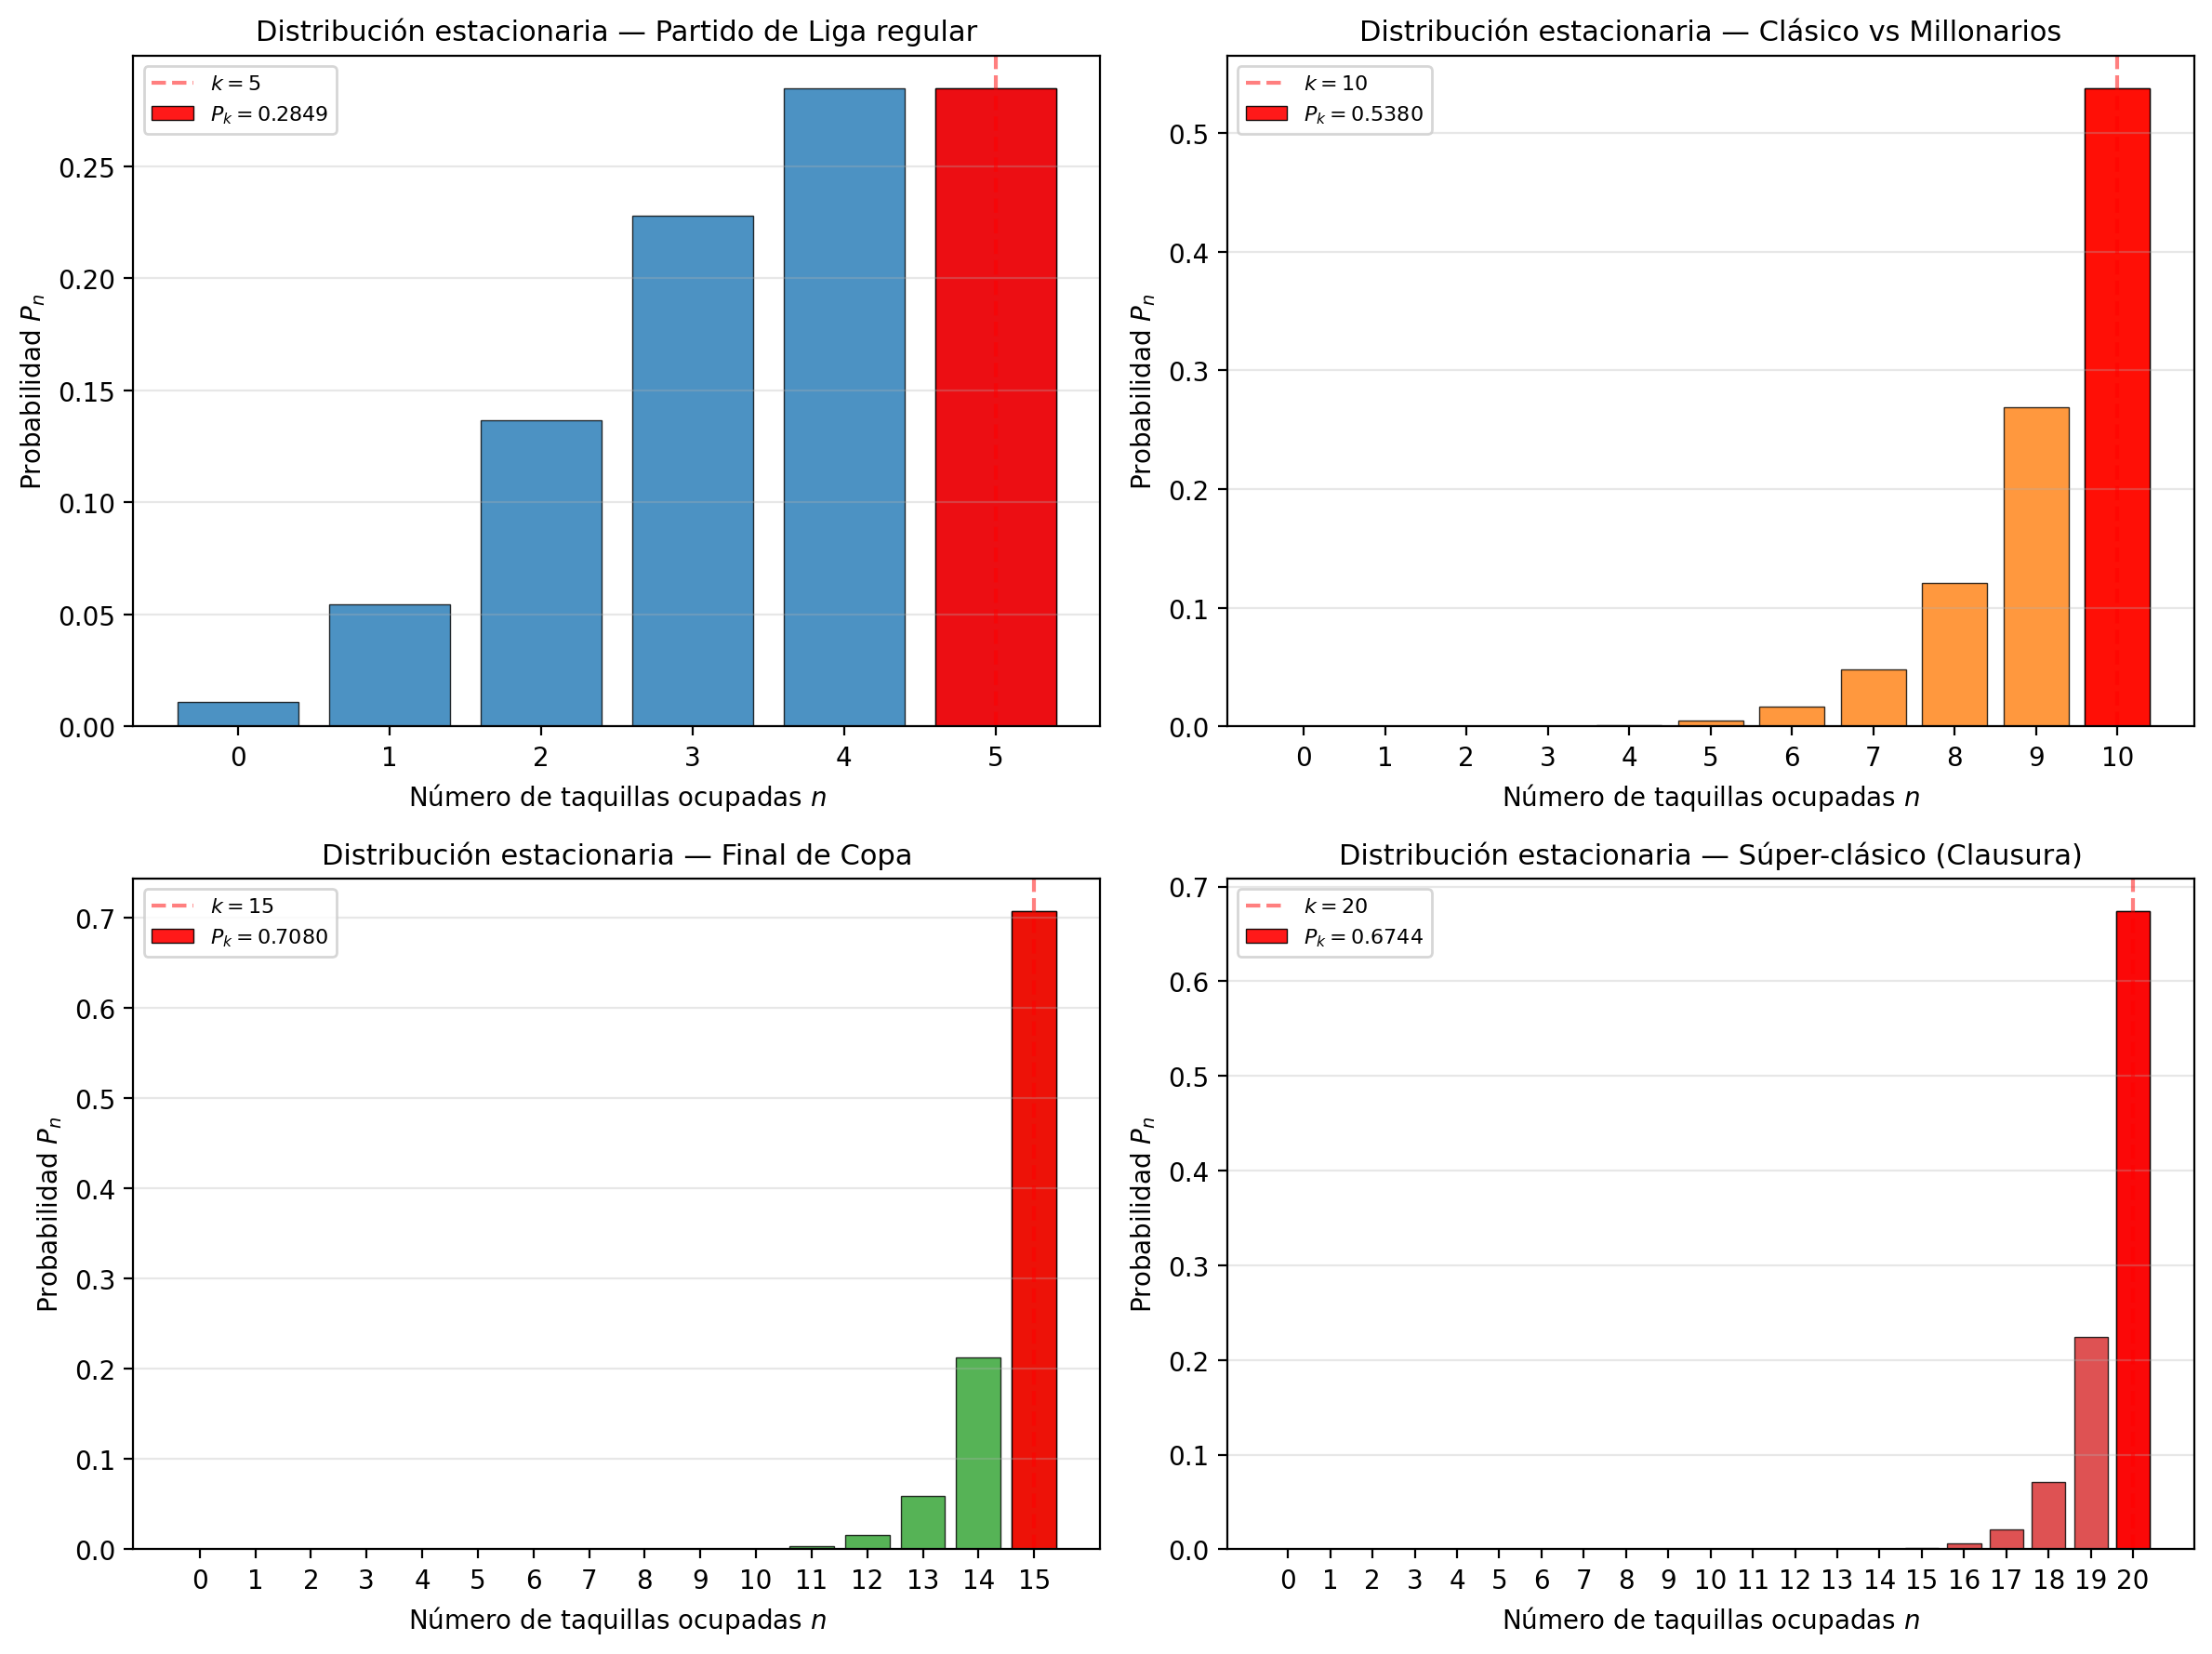
\includegraphics[width=0.98\textwidth]{plots/act_6_santafe/distribucion_estacionaria.png}
\caption{Distribución estacionaria $P_n$ para cada escenario de venta de entradas Santa Fe.
La barra roja indica $P_k$ (probabilidad de bloqueo).}
\label{fig:distribucion_tuboleta}
\end{figure}

\subsection*{Implementación}

La simulación de eventos discretos, incluyendo la generación de datos sintéticos,
la comparación entre teoría y simulación, las curvas de sensibilidad y el
dimensionamiento óptimo, fue implementada siguiendo la metodología de las
Actividades~3, 4 y~5 del curso, adaptada al contexto de la venta de entradas
para fútbol a través de una plataforma web.

% ============================================================
% FIN SECCIÓN 6 — Tu Boleta + Santa Fe
% ============================================================
